\section{The Actual Midterm Exam}
The average on this midterm exam was a 95\%. It was widely agreed to be extremely easy. Below is the grade distribution from Canvas:
\begin{figure}[H]
    \centering
    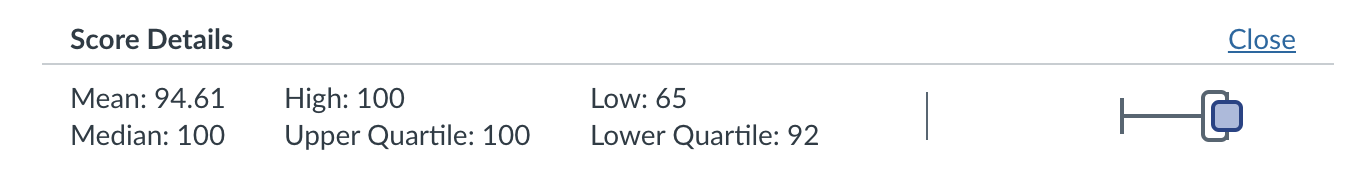
\includegraphics[width=1\linewidth]{image.png}
\end{figure}
\subsection{Problems}
Assume all functions are periodic with period 1, and let $a_n\left(\cdots\right)$ denote the Fourier coefficients of that function.
\begin{enumerate}
    \item Prove that, for $u, v \in V$ where $V$ is a real inner product space,
    \begin{align*}
        \langle u, v \rangle = \dfrac{1}{4} \left[ \norm{u+v}^2 - \norm{u-v}^2 \right]
    \end{align*}
    \item For continuous, periodic functions $f(x)$ and $g(x) := e^{6\pi ix} f(x)$, show that
    \begin{align*}
        a_n(g) = a_{n-3}(f)
    \end{align*}
    \item For continuous, periodic functions $f(x)$ and $g(x) := f(x+\frac{1}{2})$, show that
    \begin{align*}
        a_n(g) = (-1)^n \cdot a_n(f)
    \end{align*}
\end{enumerate}
\subsection{Solutions}
These solutions are transcribed from my original exam booklet, though were written up months after the course had already ended. A small amount of commentary was added because otherwise it would be too boring.
\subsubsection{Problem 1}
\begin{solution}
    We can prove this directly and quite easily:
    \begin{align}
        \dfrac{1}{4}\left( \norm{u + v}^2 - \norm{u - v}^2 \right) &= \dfrac{1}{4} \left[ \langle u+v,u+v \rangle - \langle u-v,u-v \rangle \right]
    \end{align}
    From here you could do this yourself, but we can just expand it if we don't want to expend any braincells for the other two problems which are supposedly harder.
    \begin{align}
        (13.1) &= \dfrac{1}{4} \left[ \langle u,u+v \rangle + \langle v,u+v \rangle - \langle u,u-v \rangle + \langle v,u-v \rangle \right]\\
        &= \dfrac{1}{4} \left[ \langle u,u \rangle + \langle u,v \rangle + \langle v,u \rangle + \langle v,v \rangle - \langle u,u \rangle + \langle u,v \rangle + \langle v,u \rangle - \langle v,v \rangle \right]\\
        &= \dfrac{1}{4} \left[ 2\langle u,v \rangle + 2\langle v,u \rangle \right]
    \end{align}
    Since $V$ is a real vector space,
    \begin{align}
        (13.4) = \dfrac{1}{4} \left[ 4 \langle u, v \rangle \right] = \langle u, v \rangle
    \end{align}
\end{solution}

\subsubsection{Problem 2}
\begin{solution}
    We can solve this by just writing it out and recalling how to do a substitution:
    \begin{align}
        a_n(g) &= \int_0^1 g(t) e^{-2\pi int} \dd{t}\\
        &= \int_0^1 e^{6\pi it} f(t) e^{-2\pi int} \dd{t}\\
        &= \int_0^1 f(t) e^{6\pi it -2\pi int} \dd{t}\\
        &= \int_0^1 f(t) e^{-2\pi i(n-3)t} \dd{t}\\
        &= \langle f(t), e^{2\pi i (n-3) t} \rangle\\
        &= a_{n-3}(f) \qedhere
    \end{align}
    Note that the conclusion from (13.9) to (13.10) follows from the fact that if we let
    \begin{align}
        a_m(f) = \langle f(t), e^{2\pi imt} \rangle
    \end{align}
    then set $m = n-3$ and the reasoning is trivial.
\end{solution}

\subsubsection{Problem 3}
\begin{solution}
    This is once again, a question that is solved by just writing it out:
    \begin{align}
        g(t) = f(t + 1/2) \implies a_n(g) &= \int_0^1 g(t) e^{-2\pi int} \dd{t}\\
        &= \int_0^1 f(t+1/2) e^{-2\pi int} \dd{t}
    \end{align}
    Use a substitution $u = t+1/2$ which gives $t = u-1/2$ and $\dd{t} = \dd{t}$. Then we get
    \begin{align}
        a_n(g) &= \int_{1/2}^{3/2} f(u) e^{-2\pi in(u - 1/2)} \dd{u}\\
        &= \int_{1/2}^{3/2} f(u) e^{-2\pi inu} e^{\pi in} \dd{u}\\
        &= \int_{1/2}^{3/2} (-1)^n f(u) e^{-2\pi inu} \dd{u}
    \end{align}
    Note that we leveraged the fact that $e^{\pi i n}$ equals $\pm 1$ depending on if $n$ is even or odd. After this there was some more annoying substitution, but the gist of the proof was that since $f(u)$ is periodic, we can phase shift the integral in (13.16) to be on $[0,1]$, and we get
    \begin{align}
        a_n(g) &= \int_0^1 (-1)^n  f(u) e^{2\pi in u} \dd{u}\\
        &= (-1)^n \int_0^1 f(u) e^{2\pi in u} \dd{u}\\
        &= (-1)^n a_n(f)
    \end{align}
\end{solution}
\subsection{Some notes}
I finished this in 20 minutes. It was too easy. Unfortunately for us at the time, we did not know that the final would be way harder.